
%%%%%%%%%%%%%%%%%%%%%%%%%%%%%%%%%%%%%%%%%%%%%%%%%%%%%%%%%%%%%%%%%%%%%%%%%
% SETTINGS/DEFINITIONS/CONFIGURATION
\documentclass[10pt,a4paper,titlepage,twoside]{article}
%\documentclass[10pt,a4paper,titlepage]{article}
\usepackage{ifthen}	% if else operations used for the configuration
\newboolean{German} 					% boolean for german language
\setboolean{German}{false} 		% set if german should be used, else english is
\newboolean{twosided}
\setboolean{twosided}{true}	% set if the document should be twosided
\newcommand{\defName}					% set the name of the author
	{Bastian Bechtold}
\newcommand{\defMatNr}				% set the matriculation number
	{2195907}
\newcommand{\defNameTwo}
	{Manuel Kaletta}
\newcommand{\defMatNrTwo}				% set the matriculation number
	{2076097}
\newcommand{\defSemester}			% the semester the report is created
	{SS 2013}
\newcommand{\defLocation}			% location the report was created/printed
	{Oldenburg}
\newcommand{\defInstitute}		% define the instutute/university
	{Carl von Ossietzky Universität Oldenburg}
\newcommand{\defKindOfReport}	% what the report is for (lecture/technical report/bachelor thesis)
	{Informationsverarbeitung und Kommunikation:\\
	Project Description}
\newcommand{\defTitle}				% define the title of the report
	{Sample Classification for Electronic Dance Music}

%%%%%%%%%%%%%%%%%%%%%%%%%%%%%%%%%%%%%%%%%%%%%%%%%%%%%%%%%%%%%%%%%%%%%%%%%
% PACKAGES AND SETTINGS
% language packages
\ifthenelse{\boolean{German}}
{
	\usepackage[german]{babel}
}
{
	\usepackage[english]{babel}
}

% text related
\usepackage[utf8]{inputenc}
%\usepackage[T1]{fontenc}
\usepackage{lmodern}		% changes font

% graphics related
\usepackage{graphicx}		% for graphics
%\usepackage{subfigure}	% to make subfigures
%\usepackage{epstopdf} 	% for graphics if they exist in eps

% formatting related
\usepackage{hyperref}
\usepackage{color}			% setting colors
\usepackage{fancyhdr} 	% set fancy header and footer
\fancyhead{}
\fancyfoot{}
\ifthenelse{\boolean{twosided}}
{
	\fancyhead[OL,ER] {\defTitle}
	\fancyhead[OR,EL] {\bfseries\thepage}
	\fancyfoot[OL]		{\defName, \defNameTwo}
	\fancyfoot[ER] 		{\defInstitute}
}
{
	\fancyhead[L] {\defTitle}
	\fancyhead[R] {\bfseries\thepage}
	\fancyfoot[L]	{\defName, \defNameTwo}
	\fancyfoot[R] {\defInstitute}
}
\renewcommand{\headrulewidth}{0.4pt}
\renewcommand{\footrulewidth}{0.4pt}
\usepackage{geometry}		%	set the geometry of the paper
\geometry{a4paper,left=30mm,right=30mm, top=35mm, bottom=35mm}
\usepackage{listings}		% listings environment for source code
\newcommand{\matlabinputlisting}[1][]{\lstinputlisting[language=Matlab,basicstyle=\ttfamily,#1,numbers=left,breaklines=true]}

% equations related
%\usepackage{dsfont}			% for sets
\usepackage{amsmath}		% control the Matrix like Neo
\usepackage{amstext} 		% use \text

%%%%%%%%%%%%%%%%%%%%%%%%%%%%%%%%%%%%%%%%%%%%%%%%%%%%%%%%%%%%%%%%%%%%%%%%%
% START THE DOCUMENT
\begin{document}
\pagenumbering{alph}

% cover and list of contents
\begin{titlepage}
\thispagestyle{empty}

\begin{minipage}[t]{1\textwidth}
		\vspace{-2cm}
		\hspace{-1cm}
	
\includegraphics[width=0.6\textwidth]{Pics/UniLogoBasis_Trans.pdf}
\end{minipage}

\begin{center}
\huge
\vspace{2cm}
\textsc{\defKindOfReport \\-\\ \defTitle}\\
\Large
\vspace{3cm}
\textsc{\defName \\ Mat.\-Nr: \defMatNr \\
	~\\ 
	\defNameTwo \\ Mat.\-Nr: \defMatNrTwo }\\
\vspace{1.6cm}
\textsc{\defInstitute \\ \defSemester}\\
\vfill
\large
\textsc{\defLocation, \today}
\end{center}


\end{titlepage}


\thispagestyle{empty}
\tableofcontents
\newpage

% Content of the Report
\pagenumbering{arabic}	% use arabic counting starting here
\setcounter{page}{1}		% start counting the pages here
\pagestyle{fancy} 			% start using the header and footer from here
\section{Introduction}
\label{sec:Introduction}
Electronic Dance Music (EDM) is usually built from electronic sound sources such as synthesizers or drum machines. In the last decade, more and more software products such as Digital Audio Workstations (DAW) and software instruments have been used as well. A major part of all samples are still derived from small audio snippets that are mixed into the music.\\
These samples could be base elements such as single snare hits, or whole rhythmic loops, or even complex drum arrangements. In this project, we assume that electronic dance music is comprised only of samples. Thus, complex musical productions should be representable as superpositions of many short samples. We liken these samples to words in speech in that a song is made of samples much like a sentence is made of words.\\
During the production of electronic dance music, it is often interesting to find similar samples to a known one. The process of choosing these samples can be very complex. We created an algorithm to aid in this selection process. The ideal case would be to find similar samples to all samples used in a track. \\
A conceptual framework for this would be a three step system: First, an existing collection of samples is divided into different classes. Second, short parts of a musical track are classified according to these classes. For typical tracks, there will be no clear classification, but more likely a superposition of different probabilities for each short part. Lastly, these classifications can be used to match the musical track back to the samples, thus re-synthesizing the music. In order to do this, the classes do not need to correspond to musically relevant classes such as bass drums or string instruments.\\
In this project, we are doing some basic research on this topic. We create new classes from a sample database using a clustering algorithm, and then classify test samples from these classes. Also, we classified our sample database by hand, and then classify test samples to these classes.

\section{Features}
\label{sec:Features}
Each sample is chunked into blocks. Different features are calculated on each block. The blocks have a length of 20~ms, 50~\% overlap and are Hann windowed. The remaining part of the sample, after the blocks are processed, is ignored.\\
The used features are the root mean square (RMS), peak, crest factor, spectral centroid, logarithmic spectral centroid, spectral variance, spectral skewness, spectral flatness, spectral brightness and mean spectral absolute slope. The block is given via x[k], $k$ is the frame number, the FFT of the block is X[n], $n$ is the bin number, $l$ is the number of values within one block. The features are calculated as follows:
\begin{description}
    \item[RMS:]\\
        \[
            \mathrm{RMS} = \sqrt{\frac{1}{l}\sum_{k=0}^{l}{x[k]^2}}
        \]
    \item[Peak:]\\
        \[
            \mathrm{Pk} = \max{|x[k]|}
        \]
    \item[Crest Factor:]
        \[
            \mathrm{CF} = \frac{\mathrm{Pk}}{\mathrm{RMS}}
        \]
    \item[Spectral Centroid:]
        \[
            \mathrm{SC} = \sum_{n=0}^{n=\frac{l}{2}}{X[k]\cdot \frac{n}{l}}
        \]
    \item[Spectral Variance:]
        \[
            \mathrm{SV} = \sum_{n=0}^{n=\frac{l}{2}}{}
        \]
\end{description}


The Features of each sample can be considered as a point in a $d \cdot n$ dimensional space. $d$ is the number of blocks and $d$ the number of dimensions outputted by the PCA.\\
$d$ was set to five.
\section{Distance}
\label{sec:Distance}

In order to measure the similarity of different samples, the Dynamic Time Warping (DTW) algorithm was used. DTW compares sequences of feature vectors to one another even if the sequences are of different lengths. This is important since the samples in our sample base have different lengths. DTW stretches and compresses samples feature vector sequences for maximum similarity. It can thus find similarities in samples that are elongated versions of one another or that contain each other.\\
DTW first compares every feature vector of one sample to every feature vector of another sample by calculating the euclidean distance between each feature vector. This creates a cost matrix $C$ of distances between every block of the first sample to every block of the second sample. This matrix is of dimension $N \times M$, where $N$ and $M$ are the lengths of the feature sequences of both samples, respectively.\\
Now, DTW searches for the fastest path through $C$. In order to not evaluate every possible path, DTW only calculates the cheapest path from every positive time step from $C_{n-1,m}, C_{n,m-1}, C_{n-1,m-1}$ to $C_{n,m}$. The final distance between the samples is then calculated by adding all the steps $C_{n.m}$ on the cheapest paths from $C_{0,0}$ to $C_{N,M}$. Additionally, every step is multiplied by $\frac{1}{N}$ or $\frac{1}{M}$ or $||(\frac{1}{N},\frac{1}{M})||$ to correct for the stepping distance.\\
This algorithm was implemented in Python, but found too slow for practical comparisons of big sample sets. Thus, we further implemented it in C and called that version from Python, which provided two orders of magnitude of speedup.

\section{Modified Fast Batch k-Means Algorithm}
\label{sec:TheoryKMeans}

The $k$-Means algorithm takes $k$ random points in space representing the center of $k$ classes. These class centers are then refined in two steps: First, each data point in a set of training data is classified to belong to one of the classes by selecting the closest class center. Second, the class centers are moved towards the geometric center of all the data points belonging to the class. These steps are repeated until the class centers stop moving.

However, this approach is impractical for large data sets, since every iteration needs to calculate distances from every data point to every class center. A modification of this algorithm called Mini-batch $k$-Means\footnote{http://www.eecs.tufts.edu/~dsculley/papers/fastkmeans.pdf} uses only a random subset of all data points for each iteration. This results in slightly less accurate class centers, but much greater performance.

In our case though, there is no euclidean feature space in which we could position class centers. The only measure available is the DTW-distance between the different samples. Thus, we modified the second step of the Mini-batch $k$-Means algorithm to choose the centermost sample instead of an arbitrarily chosen point. The centermost sample is defined as the one sample in the class that has the least distance to all other samples in the class.

Running this algorithm on our data set results in $k$ class centers. New samples can then be classified to belong to one of these centers by selecting the closest one.

Calculating class centers requires the calculation of many distances between many samples. In order to speed up this process, all distances between all samples have been pre-calculated and put into a database. This process can take several hours on modern computers\footnote{about 1.5 hours on quad-core Unix, or 6 hours on Windows}. The class centers are then calculated based on the distances in this database. We used a Pandas DataFrame to represent the database.

\section{$k$-Nearest-Neighbors Algorithm}
\label{sec:TheoryKnn}
The $k$-Nearest-Neighbors ($k$-NN) algorithm performs a distribution free classification task. It uses a lazy learning approach which means that all the training data is saved. The Algorithm searches that data base for the $k$ closest data points to the point to classify. The distance measurement depends on the application. The class which is most often found in those $k$ nearest neighbors is the one the sample is classified as \cite[p.~338~f.]{bib:Alzate2007}.\\
The space of the data points is the PCA-reduced feature space described in section~\ref{sec:Features}. The distance used in our project is the DTW-distance described in section~\ref{sec:Distance}. The feature space version of a test sample is calculated and compared to all other feature vectors in the database from section~\ref{sec:Features}. This comparison table is then sorted by distance using the sorting algorithm built into Python. As output of the $k$-NN classification, the ratio of found neighbors to the total number of neighbors is given for the $k$ nearest neighbors. This can be interpreted as the probability of a point belonging to a class.

\section{Measurements and Results}
\label{sec:Measurements}
A test sample base was created with ten tracks for each class. All of the test samples were new samples that were not included in the training sample base.

\subsection{Modified Mini Batch $k$-Means}
The $k$-Means algorithm was used to calculate $k=10$ class centers in our sample base using a batch size of 500 points and 50 iterations. These classes were used to classify our test sample base. The tags of the test samples within each of the 10 class clusters created by the $k$-Means algorithm were counted. The results are shown in figure~\ref{fig:k-Means}.\\
It can be seen that the algorithmically calculated classes do not correspond well to the tags defined by our sample base. In eight different measurements the percentage of right classified samples was 23~\% in the mean, minimum 8.3~\% and maximum 33.3~\%. Such modest results were to be expected. Nevertheless, it seems that there are some consistent mappings in the structuring of the tags. This needs to be verified with further research. % 28, 30, 34, 40, 10, 10, 37, 34 of 120
\begin{figure}[htbp]
\centering
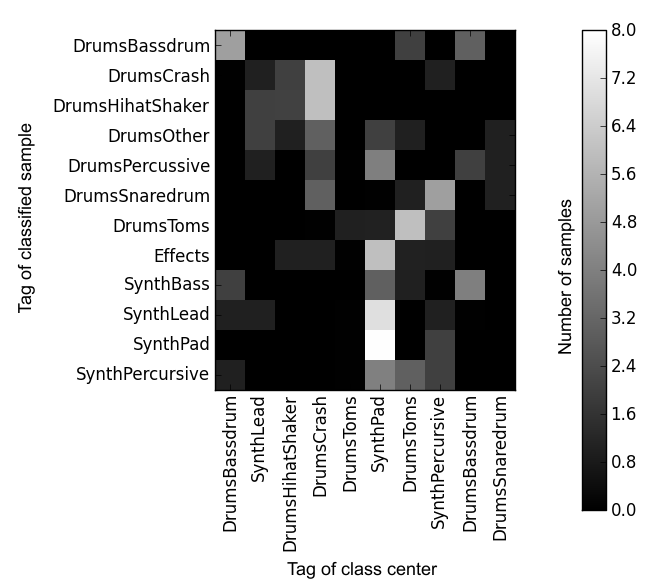
\includegraphics[width=0.45\linewidth]{../measurements/k_means_1_mod.png}
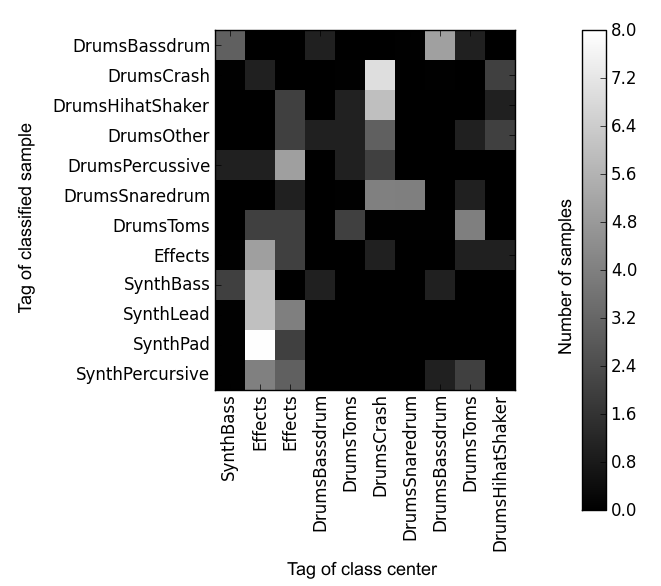
\includegraphics[width=0.45\linewidth]{../measurements/k_means_2_mod.png}
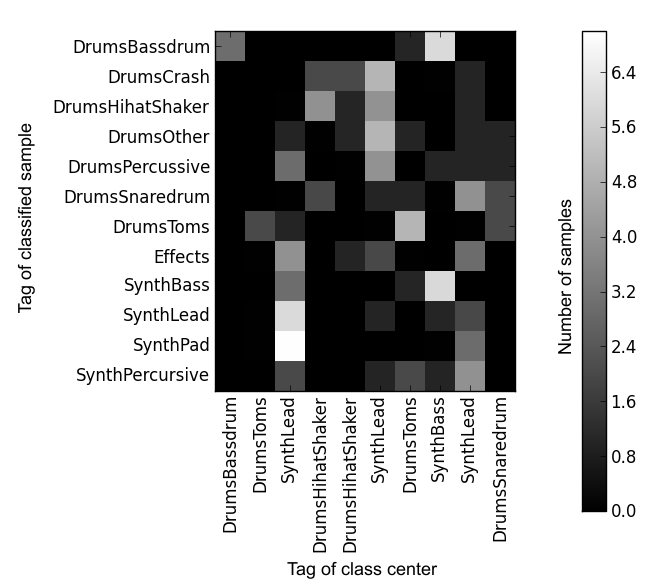
\includegraphics[width=0.45\linewidth]{../measurements/k_means_3_mod.png}
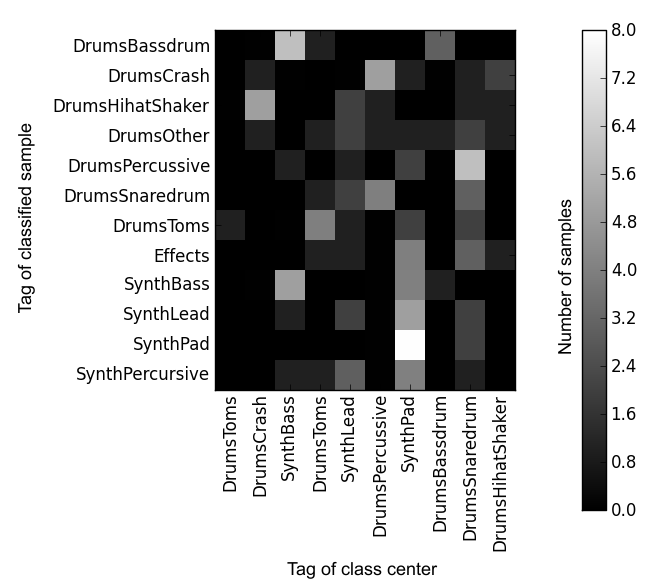
\includegraphics[width=0.45\linewidth]{../measurements/k_means_4_mod.png}
\caption{Number of samples, depending on their tag and the tag of the class center they were assigned to. The 10 classes were generated by a modified mini batch $k$-Means algorithm with a batch size of 500 using 50 iterations. The four plots represent four different runs of the modified mini batch $k$-Means algorithm.}
\label{fig:k-Means}
\end{figure}

\subsection{$k$-Nearest-Neighbors}
All the samples in the test sample bank were classified using the implemented $k$-NN algorithm with $k=10$. The results are shown in figure~\ref{fig:k-NN}. The tags of the test bank are plotted against the tags of the classification.\\
The results show that many of the samples are classified correctly. The percentage of correct classified samples is 48.3~\%. This even exceeds our expectations. The variations in the classification correlate with the variances between samples of the same tag in the sample base. This means that the classes that are badly classified are also hard to classify by human perception.
%right class hits:  58
%wrong class hits:  62
%percentage right:  48.333333333333336

\begin{figure}[htbp]
\centering
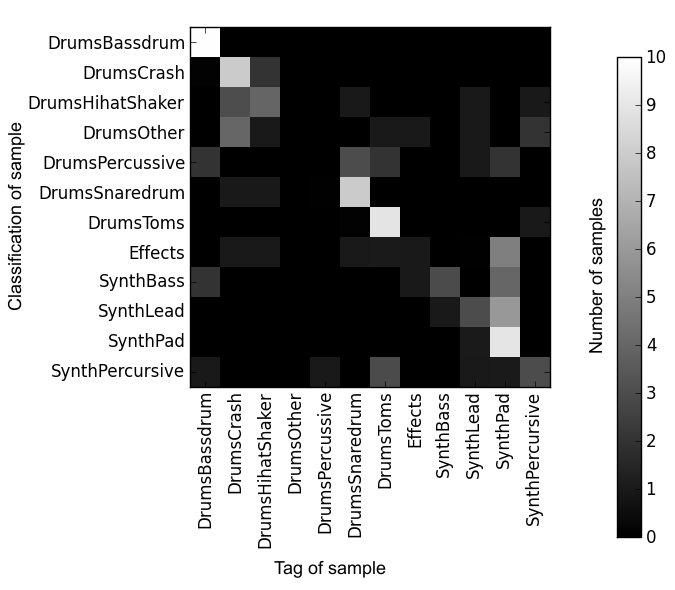
\includegraphics[width=0.47\linewidth]{../measurements/knn_mod.png}
\caption{Number of Samples, depending on their tag and the assigned tag by the $k$-NN algorithm with $k=10$.}
\label{fig:k-NN}
\end{figure}

\subsection{Nearest-Neighbor}
Also solely the nearest neighbor was searched, to get a sample in the training sample base that should be similar to the test sample. This measurement shows that the current system already has some application on the aimed usage.\\
A pre-listening test on the results shows that they give a useful selection sometimes but that the selected samples are still too dissimilar in most cases.



\section{Discussion}
A classification of audio samples was performed using two approaches. The results on the clustering show that the automatic cluster differ strongly from the human sorted classes. Nevertheless the classification of samples based directly on the human sorting showed quite good results. Consequently the task of assigning samples is possible and further research on this has the potential of much improvement.\\
One big area of open research are the features. More and/or better features could give a much better differentiation of the samples. Also a listening test for measuring the perceived distance in between samples could be done. This could then be used to check how good the perceived differences correlate with the distances the algorithm calculates.

% Begin Appendix
\newpage
\begin{appendix}
%\section[Derivation]{Some Derivation}
%\label{appendix:Derivation}
%\begin{equation}
%\label{eq:difficultLookingEquation}
%\begin{pmatrix}
%	x_u^2 & x_u & 1 \\ x_m^2 & x_m & 1 \\x_o^2 & x_o & 1
%\end{pmatrix} 
%\cdot 
%\begin{pmatrix} 
%a \\ b \\ d\end{pmatrix} 
%= 
%\begin{pmatrix} 
%y_1 \\ y_2 \\ y_3
%\end{pmatrix}
%\end{equation}

								% own appendix
\newpage

\bibliographystyle{alpha}
\bibliography{Bibliography}
\ifthenelse{\boolean{German}}
{
	\addcontentsline{toc}{section}{Literatur}
}
{
	\addcontentsline{toc}{section}{References}
}
\end{appendix}

\end{document}
